

\section{Evaluation}
\subsection{Setup}

\noindent\textbf{Evaluation Datasets}. We evaluate {\sysname} on diverse  mathematical benchmarks.  In addition to the widely-used  GSM8K~\citep{gsm8k}, we include challenging benchmarks from multiple domains: \textit{(i)} competition and Olympiad-level benchmarks, such as MATH-500~\citep{lightman2023let}, AIME 2024~\citep{aime}, AMC 2023~\citep{amc} and Olympiad Bench~\citep{he2024olympiadbench}. Specifically,  AIME is the exams designed to challenge the brightest high school math students in American, with the 2024 dataset comprising 30 problems from AIME I and II exams; 
\textit{(ii)} college-level math problems from College Math~\citep{mathscale} and \textit{(iii)} out-of-domain math benchmark: GaoKao (Chinese
College Entrance Exam) En 2023~\citep{liao2024mario}. 






\noindent\textbf{Base Models and Setup}. {\sysname} is a general approach applicable to various LLMs. To show its effectiveness and generalizability, we use SLMs of different sizes as the base policy models:  
Qwen2.5-Math-1.5B~\citep{qwen2.5-math-1.5b}, Phi3-mini-Instruct (3B)~\citep{phi3-4k,phi3}, Qwen2-Math-7B~\citep{qwen2-math-7b} and Qwen2.5-Math-7B~\citep{qwen2.5-math-7b}. Among these, Phi3-mini-Instruct is a general-purpose SLM without specialization in math reasoning. 

Due to limited GPU resources, we performed 4 rounds of self-evolution exclusively on Qwen2.5-Math-7B, yielding 4 evolved policy SLMs (Table~\ref{tbl:policyllm}) and 4 PPMs (Table~\ref{tbl:prm-evolution}). For the other 3 policy LLMs, we fine-tune them using step-by-step verified trajectories generated from  Qwen2.5-Math-7B's 4th round. The final PPM from this round is then used as the reward model for the 3 policy SLMs. 







\noindent\textbf{Baselines}.  {\sysname} is a System 2 method. We compare it against three strong baselines representing both System 1 and System 2 approaches: \textbf{(i)} \textit{Frontier LLMs}, including GPT-4o, the latest Claude, OpenAI o1-preview and o1-mini. 
 We measure their accuracy on AMC 2023, Olympiad Bench, College Math, Gaokao and GSM8K, with accuracy numbers for other benchmarks are taken from public technical reports~\citep{qwq-32b-preview}. 
\textbf{(ii)} \textit{Open-sourced superior reasoning models}, including DeepSeek-Coder-v2-Instruct, Mathstral~\citep{mathstral}, NuminaMath-72B~\citep{numina_math_datasets}, and LLaMA3.1~\citep{llama3.1}, which represent the current mainstream System 1 approaches for improving LLM math reasoning. \textbf{(iii)} \textit{Both System 1 and System 2 performance of the base models trained from the original models teams}, including Instruct versions (e.g., Qwen2.5-Math-7B-Instruct) and  Best-of-N (e.g., Qwen2.5-Math-72B-Instruct+Qwen2.5-Math-RM-72B).  Notably, the reward model used for the three Qwen base models is a 72B ORM, significantly larger than our 7B PPM.


\noindent\textbf{Evaluation Metric}. We report Pass@1 accuracy for all baselines. For System 2 baselines, we use default evaluation settings, such as default thinking time for o1-mini and o1-preview. For  Qwen models with Best-of-N, we re-evaluate  MATH-500, AIME/AMC accuracy; other benchmarks results are from their technical reports. For a fair comparison, {\sysname} run MCTS to generate the same number of solutions as Qwen. Specifically, for AIME/AMC, we generate 16 trajectories for AIME/AMC and 8 for other benchmarks, using PPM to select the best solution. We also report performance with increased test-time computation using 64 trajectories, denoted as {\sysname}$^{64}$.




\begin{table*}[t]
	\small 
	\centering
	\caption{The results of {\sysname} and other frontier LLMs on the most challenging math benchmarks. \sysname$^{64}$ shows the Pass@1 accuracy achieved when sampling 64 trajectories. }
	\label{tbl:mainresults}
	\resizebox{1\textwidth}{!}{
		\begin{tabular}%{@{\hskip0pt}c@{\hskip4pt}|cccc@{\hskip0pt}}
			{@{\hskip0pt}l@{\hskip4pt}c@{\hskip6pt}c@{\hskip6pt}c@{\hskip6pt}c@{\hskip6pt}c@{\hskip6pt}c@{\hskip6pt}c@{\hskip6pt}c@{\hskip0pt}}
			\toprule[1.5pt]
			&&  \multicolumn{4}{c}{\bf Competition and College Level} &  && \bf OOD \\
			\cmidrule{3-7} 
			Model&Method&MATH &\makecell{AIME\\2024} & \makecell{AMC\\2023}& \makecell{Olympiad \\Bench}&\makecell{College\\Math}&GSM8K&\makecell{Gaokao\\En 2023}\\
			\midrule[1pt]
		  \multicolumn{9}{l}{\textit{Frontier LLMs}}\\
		  GPT-4o&System 1&76.6&9.3&47.5&43.3&48.5& 92.9&67.5\\
		  Claude3.5-Sonnet&System 1& 78.3& 16.0& -&-&- &96.4 &- \\
		  GPT-o1-preview&-& 85.5  &44.6&90.0& -&-&  -&- \\
		  GPT-o1-mini &- &\underline{\textbf{90.0}}&\underline{\textbf{56.7}}&\underline{\bf95.0 }&\underline{\bf{65.3}} &57.8&94.8&78.4  \\
		  	\midrule[1pt]
	  \multicolumn{9}{l}{\textit{Open-Sourced Reasoning LLMs}}\\
		  DeepSeek-Coder-V2-Instruct&System 1&75.3&13.3&57.5&37.6&46.2& 94.9&64.7\\
		  Mathstral-7B-v0.1&System 1&57.8&0.0&37.5&21.5&33.7& 84.9& 46.0\\
		 NuminaMath-72B-CoT&System 1&64.0&3.3&70.0&32.6&39.7&90.8& 58.4\\
		  LLaMA3.1-8B-Instruct &System 1& 51.4&6.7 &25.0& 15.4& 33.8& 76.6&38.4\\
		  LLaMA3.1-70B-Instruct & System 1&65.4&23.3&50.0&27.7&42.5&94.1&54.0\\
		   Qwen2.5-Math-72B-Instruct&System 1 &85.6&30.0&70.0&49.0&49.5&95.9&71.9\\
		   Qwen2.5-Math-72B-Instruct+72B ORM&System 2 &85.8&36.7&72.5&54.5&50.6&96.4&76.9\\
		  	\midrule[1pt]
		  \multicolumn{9}{c}{\textit{General Base Model: Phi3-mini-Instruct (3.8B)}}\\
		  Phi3-mini-Instruct (base model)& System 1 & 41.4&3.33&7.5&12.3&33.1&85.7& 37.1   \\
	\rowcolor{airforceblue}	   \textbf{{\sysname} (3.8B SLM+7B PPM)} &System 2 &\bf 85.4&\bf 40.0&\bf 77.5&\bf59.3&\underline{\bf58.0}&\bf94.5&\bf77.1\\
		\rowcolor{airforceblue}	   \textbf{{\sysname}$^{64}$ (3.8B SLM+7B PPM)} &System 2 &\bf 86.4&\bf 43.3&\bf 80.0&\bf60.3&\underline{\bf59.1}&\bf94.7&\bf77.7\\
		\midrule[1pt]
		 \multicolumn{9}{c}{\textit{Math-Specialized Base Model: Qwen2.5-Math-1.5B}}\\
	Qwen2.5-Math-1.5B (base model)&System 1	 &51.2 &0.0&22.5&16.7&38.4& 74.6& 46.5   \\
	Qwen2.5-Math-1.5B-Instruct &System 1&60.0&10.0& 60.0&38.1&47.7& 84.8&65.5\\
	Qwen2.5-Math-1.5B-Instruct+72B ORM &System 2 & 83.4&20.0&72.5& 47.3& 50.2& 94.1& 73.0\\
	\rowcolor{airforceblue} \textbf{{\sysname} (1.5B SLM+7B PPM)} &System 2 &\bf87.8&\bf 46.7&\bf 80.0&\bf63.5&\underline{\bf59.0}&\bf 94.3&\bf77.7\\
	\rowcolor{airforceblue} \textbf{{\sysname}$^{64}$ (1.5B SLM+7B PPM)} &System 2 &\bf88.6&\bf 46.7&\bf 85.0&\bf64.6&\underline{\bf59.3}&\bf 94.8&\underline{\bf79.5}\\
		\midrule[1pt]
		\multicolumn{9}{c}{\textit{Math-Specialized Base Model: Qwen2-Math-7B}}\\
		Qwen2-Math-7B (base model)& System 1 & 53.4&3.3& 25.0&17.3&39.4&80.4&47.3    \\
		Qwen2-Math-7B-Instruct& System 1 & 73.2&13.3&62.5&38.2& 45.9&89.9& 62.1 \\
		Qwen2-Math-7B-Instruct+72B ORM& System 2 &83.4&23.3&62.5&47.6&47.9&\bf 95.1&71.9\\
		\rowcolor{airforceblue} \textbf{{\sysname} (7B SLM+7B PPM)} &System 2 &\bf88.2&\bf 43.3&\bf 80.0&\bf 63.1&\underline{\bf58.4}&94.6&\bf78.2\\
			\rowcolor{airforceblue} \textbf{{\sysname}$^{64}$ (7B SLM+7B PPM)} &System 2 &\bf88.6&\bf 46.7&\bf 85.0&\bf 63.4&\underline{\bf59.3}&94.8&\underline{\bf79.2}\\
		\midrule[1pt]
		\multicolumn{9}{c}{\textit{Math-Specialized Base Model: Qwen2.5-Math-7B}}\\
			Qwen2.5-Math-7B (base model)&System 1 & 58.8 &0.0&22.5&21.8&41.6& 91.6&51.7    \\
	  Qwen2.5-Math-7B-Instruct& System 1& 82.6 &6.0&62.5&41.6& 46.8& 95.2& 66.8 \\
	 Qwen2.5-Math-7B-Instruct+72B ORM&System 2 &88.4&26.7&75.0&49.9&49.6&\underline{\bf97.9 }&75.1\\
\rowcolor{airforceblue}	 \textbf{{\sysname} (7B SLM+7B PPM)} &System 2 &\bf 89.4&\bf 50.0&\bf 87.5&\underline{\bf65.3}&\underline{\textbf{59.0}}&95.0&\underline{\textbf{80.5}}\\
\rowcolor{airforceblue}	 \textbf{{\sysname}$^{64}$ (7B SLM+7B PPM)} &System 2 &\underline{\bf 90.0}&\bf 53.3&\bf 87.5&\underline{\bf65.6}&\underline{\textbf{60.5}}&95.2&\underline{\textbf{81.3}}\\
				\midrule[1pt]
	\end{tabular}}
\end{table*}





\subsection{Main Results}

\noindent\textbf{Results on diverse challenging math benchmarks}. Table~\ref{tbl:mainresults} shows the results of {\sysname} with comparing to state-of-the-art reasoning models. We highlight three key observations: \textbf{(1)} {\sysname} significantly improves SLMs math reasoning capabilities,  achieving performance comparable to or surpassing OpenAI o1 with substantially smaller model size (1.5B-7B). For example, Qwen2.5-Math-7B, originally at 58.8\% accuracy on MATH, improved dramatically to 90.0\% with {\sysname}, outperforming o1-preview and Claude 3.5 Sonnet while matching o1-mini. On the College Math benchmark, {\sysname} exceeds o1-mini by 2.7\%. On AIME 2024, {\sysname} scored 53.3\%, ranking just below o1-mini, with the 7B model solving 8/15 problems in both AIME I and II, placing in the top 20\% of the brightest high school math students.
 Notably, 8 of the unsolved problems were geometry-based, requiring visual understanding, a capability  {\sysname}currently does not support.  \textbf{(2)} Despite using smaller policy models (1.5B-7B) and reward models (7B), {\sysname} significantly outperforms state-of-the-art System 2 baselines. Compared to Qwen Best-of-N baselines, which use the same base models (Qwen2-Math-7B, Qwen2.5-Math-1.5B/7B) but a 10$\times$ larger reward model  (Qwen2.5-Math-RM-72B), {\sysname} consistently improves the reasoning accuracy of all base models to state-of-the-art levels. Even against Best-of-N with a 10$\times$ larger Qwen2.5-Math-72B-Instruct policy model, {\sysname} surpasses it on all benchmarks except GSM8K, using the same number of sampled solutions. 
 \textbf{(3)} Beyond well-known benchmarks like MATH, GSM8K, and AIME, which may risk over-optimization, {\sysname} shows strong generalizability on other challenging math benchmarks, including Olympiad Bench, College Math, and the Chinese College Entrance Math Exam (Gaokao), setting new state-of-the-art scores. As discussed in Sec.~\ref{sec:selfevolution}, our training set is primarily sourced from public datasets, with no specific optimizations for these benchmarks.


\begin{figure*}[ht]
	\centering
	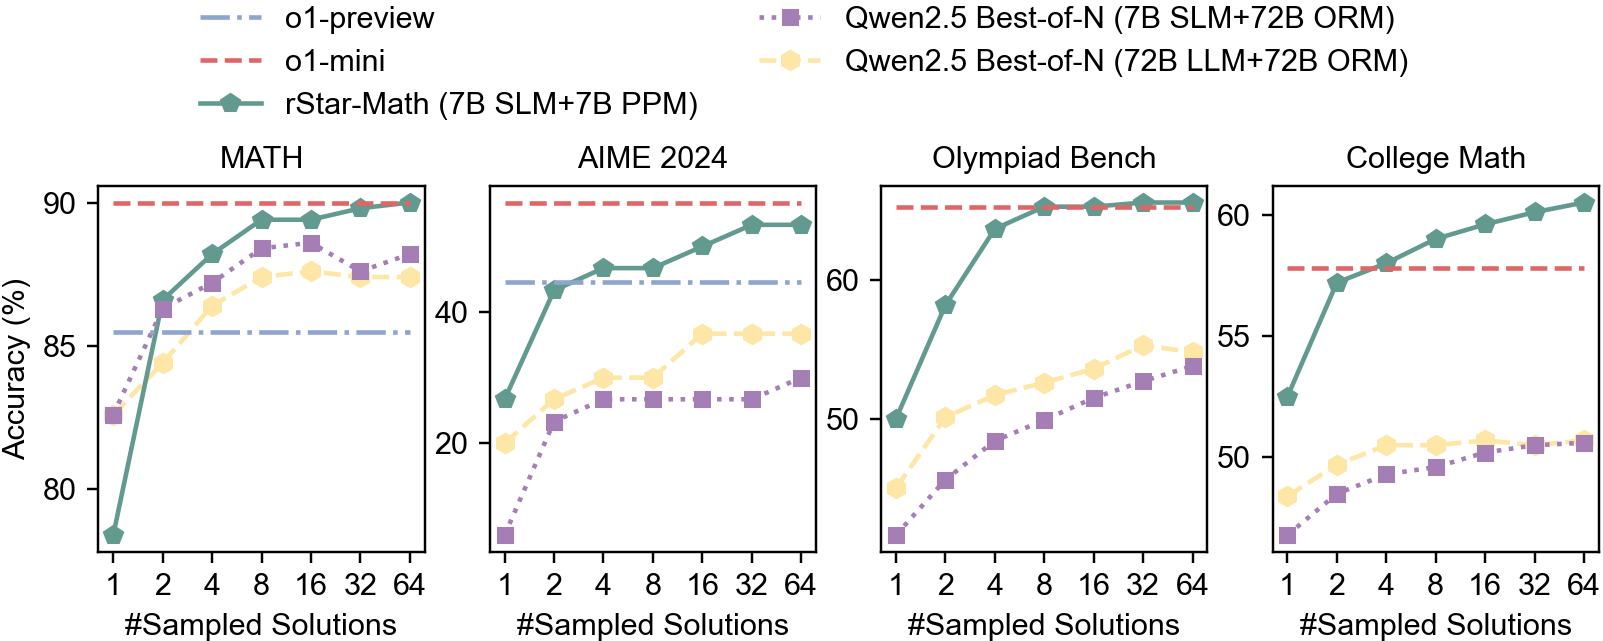
\includegraphics[width=1\textwidth]{scalinglaws.png}
	\vspace{-3ex}
	\caption{Reasoning performance under scaling up the test-time compute. }
	\label{fig:scalinglaws}
\end{figure*}


\noindent\textbf{Scaling up test-time computation}. {\sysname} uses MCTS to augment the policy model, searching solutions guided by the PPM.  By increasing test-time computation, it explores more trajectories, potentially improving performance.
 In Fig.~\ref{fig:scalinglaws}, we show the impact of test-time compute scaling by comparing the accuracy of the official Qwen Best-of-N across different numbers of sampled trajectories on four challenging math benchmarks. Sampling only one trajectory corresponds to the policy LLM's Pass@1 accuracy,  indicating a fallback to System 1 reasoning.  We highlight two key observations: \textbf{(1)} With only 4 trajectories, {\sysname} significantly outperforms Best-of-N baselines, exceeding o1-preview and approaching o1-mini, demonstrating its effectiveness. \textbf{(2)} Scaling test-time compute improves reasoning accuracy across all benchmarks, though with varying trends. On Math, AIME, and Olympiad Bench, {\sysname} shows saturation or slow improvement at 64 trajectories, while on College Math, performance continues to improve steadily.
\subsection{Ablation Study and Analysis}
We ablate the effectiveness of our three innovations. For System 2-style inference, Pass@1 accuracy is measured with 16 trajectories for AIME and AMC, and 8 for other benchmarks.
 
\begin{table*}[hpt]
	\small 
	\centering
	\caption{The continuously improved math reasoning capabilities through {\sysname} self-evolved deep thinking. Starting from round 2, the 7B base model  powered by {\sysname} surpasses GPT-4o. }
	\label{tbl:self-evolution}
	\resizebox{1\textwidth}{!}{
		\begin{tabular}%{@{\hskip0pt}c@{\hskip4pt}|cccc@{\hskip0pt}}
			{cccccccc}
			\toprule
			Round\#&MATH&AIME 2024& AMC 2023& Olympiad Bench& College Math&GSM8K&GaokaoEn 2023  \\
			\midrule 
				GPT-4o&76.6&9.3&47.5&43.3&48.5& 92.9&67.5\\
				\midrule 
			Base 7B model & 58.8&0.0&22.5&21.8&41.6&91.6&51.7\\
			{{\sysname} Round 1} &75.2 &10.0 &57.5&35.7&45.4& 90.9&60.3 \\
			{{\sysname}	Round 2} &86.6 &43.3& 75.0&59.4&55.6& 94.0&76.4   \\
			 {{\sysname}	Round 3} &87.0 & 46.7&80.0& 61.6&56.5& 94.2& 77.1   \\
			 {{\sysname}	Round 4} &\bf 89.4  &\bf 50.0  &\bf 87.5 &\bf 65.3 &\bf 59.0 &\bf 95.0 &\bf  80.5\\
			\hline
	\end{tabular}}
	%	\vspace{-1ex}
\end{table*}


\noindent\textbf{The effectiveness of self-evolution}.  The impressive results in Table~\ref{tbl:mainresults} are achieved after 4 rounds of {\sysname} self-evolved deep thinking. Table~\ref{tbl:self-evolution} shows the math reasoning performance in each round, demonstrating a continuous improvement in  accuracy. 
 In round 1, the main improvement comes from applying SFT to the base model. Round 2 brings a significant boost with the application of a stronger PPM in MCTS, which unlocks the full potential of System 2 deep reasoning. Notably, starting from round 2,  {\sysname} outperforms GPT-4o. Rounds 3 and 4 show further improvements, driven by stronger System 2 reasoning through better policy SLMs and PPMs. 


\noindent\textbf{The effectiveness of step-by-step verified reasoning trajectory}.  {\sysname} generates step-by-step verified reasoning trajectories,  which eliminate error intermediate steps and further expand training set with more  challenging problems. To evaluate its effectiveness, we use the data generated from round 4  as SFT training data and compare it against 
 three strong baselines: \textit{(i)} GPT-distillation, which includes open-sourced CoT solutions synthesized using GPT-4, such as MetaMath~\citep{yu2023metamath}, NuminaMath-CoT~\citep{numinamathcot}; \textit{(ii)} Random sampling from self-generation, 
 which use the same policy model (i.e., policy SLM-r3) to randomly generate trajectories; \textit{(iii)} Rejection sampling, where 32 trajectories are randomly sampled from the policy model, with high-quality solutions ranked by our trained ORM (appendix~\ref{sec:appendexp}). For fairness, we select two correct trajectories for each math problem in baseline (ii) and (iii). All SFT experiments use the same training recipe.
 
 

\begin{table*}[hpt]
	\small 
	\centering
	\caption{Ablation study on the effectiveness of our step-by-step verified reasoning trajectories as the SFT dataset. We report the SFT accuracy  of Qwen2.5-Math-7B fine-tuned with different datasets.  }
	\label{tbl:datacompare}
	\resizebox{1\textwidth}{!}{
		\begin{tabular}%{@{\hskip0pt}c@{\hskip4pt}|cccc@{\hskip0pt}}
			{@{\hskip0pt}c@{\hskip2pt}c@{\hskip2pt}c@{\hskip6pt}c@{\hskip6pt}c@{\hskip6pt}c@{\hskip6pt}c@{\hskip6pt}c@{\hskip6pt}c@{\hskip0pt}}
			\toprule
			&Dataset&MATH&AIME& AMC& Olympiad Bench& College Math&GSM8K&GaokaoEn 2023 \\
			\midrule 
			
				GPT-4o&-&76.6&9.3&47.5&43.3&48.5& \bf92.9&\bf67.5\\
				 \midrule
		\multirow{2}{*}{\makecell{GPT4-distillation\\ (Open-sourced)}}	& MetaMath&55.2  & 3.33 & 32.5& 19.1& 39.2& 85.1& 43.6\\
		&	NuminaMath-CoT & 69.6 &10.0  &\bf50.0 &37.2 &43.4 &89.8 &59.5 \\
			 \midrule
\multirow{3}{*}{\makecell{Self-generation\\ by policy SLM-r3}}			&	Random sample & 72.4 &10.0  & 45.0&41.0 &48.0 &87.5 &57.1 \\
	&		Rejection sampling & 73.4 & 13.3 &47.5 & 44.7& 50.8&89.3&61.7\\
		&	\bf Step-by-step verified (ours)  & \bf78.4& \bf 26.7 & 47.5&\bf 47.1 &  \bf 52.5&89.7 & 65.7\\
			\hline
	\end{tabular}}
	%	\vspace{-1ex}
\end{table*}
Table~\ref{tbl:datacompare} shows the math reasoning accuracy of Qwen2.5-Math-7B fine-tuned on different datasets. We highlight two observations: \textbf{(i)} Fine-tuning with our step-by-step verified trajectories significantly outperforms all other  baselines. This is primarily due to our PPM-augmented MCTS for code-augmented CoT  synthesis,  which provides denser verification during math solution generation. It proves more effective than both random sampling, which lacks verification,  and rejection sampling, where ORM provides only sparse verification. \textbf{(ii)} Even randomly sampled code-augmented CoT solutions from our SLM yields comparable or better performance than GPT-4 synthesized NuminaMath and MetaMath datasets. 
 This indicates that our policy SLMs, after rounds of self-evolution, can generate high-quality math solutions.  These results demonstrates the huge potential of our method to self-generate higher-quality reasoning data without relying on advanced LLM distillation. 
 

\noindent\textbf{The effectiveness of PPM}. We train both a strong ORM and Q-value score-based PRM (PQM) for comparison. To ensure a fair evaluation, we use the highest-quality training data: the step-by-step verified trajectories generated in round 4, with selected math problems matching those used for PPM training.  Similar to PPM, we use step-level Q-values as  to select positive and negative trajectories for each math problem. 
The ORM is trained using a pairwise ranking loss~\citep{instructgpt}, while the PQM follows~\citep{alphamath,restmcts} to use Q-values as reward labels and optimize with MSE loss. Detailed training settings are provided in Appendix~\ref{sec:appendexp}.

\begin{table*}[hpt]
	\small 
	\centering
	\caption{Ablation study on the reward model. Process reward models (PQM and PPM) outperform ORM, with PPM pushing the frontier of math reasoning capabilities.}
	\label{tbl:rmablation}
	\resizebox{1\textwidth}{!}{
		\begin{tabular}%{@{\hskip0pt}c@{\hskip4pt}|cccc@{\hskip0pt}}
			{ccccccccc}
			\toprule
			RM&Inference &MATH&AIME& AMC& Olympiad Bench& College Math&GSM8K&GaokaoEn     \\
			\midrule
			 o1-mini &- &\underline{\textbf{90.0}}&\underline{\textbf{56.7}}&\underline{\bf95.0 }&\underline{\bf{65.3}} &55.6&94.8&78.6  \\
			 \midrule
		ORM&Best-of-N&82.6  &26.7  &65.0 & 55.1&55.5 &92.3 &72.5 \\
				PQM &MCTS&88.2  & 46.7 & 85.0& 62.9& \underline{\bf57.6}&94.6&\underline{\bf79.5} \\
				PPM &MCTS&\bf 89.4  &\bf 50.0  &\bf 87.5 &\underline{\bf 65.3}&\underline{\bf 59.0} &\underline{\bf 95.0} &\underline{\bf  80.5} \\
			\hline
	\end{tabular}}
		\vspace{-1ex}
\end{table*}




Table~\ref{tbl:rmablation} compares the performance of  ORM, PQM, and PPM for System 2 reasoning using our final round policy model. ORM provides reward signals only at the end of problem solving, so we use the Best-of-N method, while PRM and PPM leverage MCTS-driven search.  As shown in Table~\ref{tbl:rmablation}, both PQM and PPM outperform ORM by providing denser step-level reward signals, leading to higher accuracy on complex math reasoning tasks. However, PQM struggles on more challenging benchmarks, such as MATH and Olympiad Bench,  due to the inherent imprecision of Q-values.
In contrast, PPM constructs step-level preference data for  training, enabling our 7B policy model to achieve comparable or superior performance to o1-mini across all benchmarks.














\section{Findings and Discussions} 

\begin{figure*}[ht]
	\centering
	\includegraphics[width=1\textwidth]{self-reflection3.pdf}	
	\vspace{-3ex}
	\caption{An example of intrinsic self-reflection during {\sysname} deep thinking.}
	\label{fig:selfcorrect}
\end{figure*}


 \noindent\textbf{The emergence of intrinsic self-reflection capability}. A key breakthrough in OpenAI  o1 is its intrinsic self-reflection capability. When the model makes an error, it recognizes the mistake and can  self-correct with a correct answer~\citep{o1backtracing}. Yet it has consistently 
 been found to be largely ineffective in open-sourced LLMs. The community has actively explored various approaches, including self-correction~\citep{huang2023large,kumar2024training}, self-reflection~\citep{renze2024self,shinn2024reflexion},  to explicitly train or prompt LLMs to develop  such capability. 


 
 In our experiments, we unexpectedly observe that our  MCTS-driven deep thinking  exhibits self-reflection during  problem-solving.  As shown in Fig.~\ref{fig:selfcorrect}, the model initially formalizes an equation using \texttt{SymPy} in the first three steps, which would lead to an incorrect answer (left branch). Interestingly, in the fourth step (right branch), the policy model recognizes the low quality of its earlier steps and refrains from continuing along the initial problem-solving path. Instead, it backtracks and resolves the problem using a new, simpler approach, ultimately arriving at the correct answer. An additional example of self-correction is provided in Appendix\ref{sec:trajectoryexample}. Notably, no self-reflection training data or prompt was included, suggesting that advanced System 2 reasoning can foster intrinsic self-reflection.
 

 
 
 

 
\begin{figure*}[ht]
	\centering
	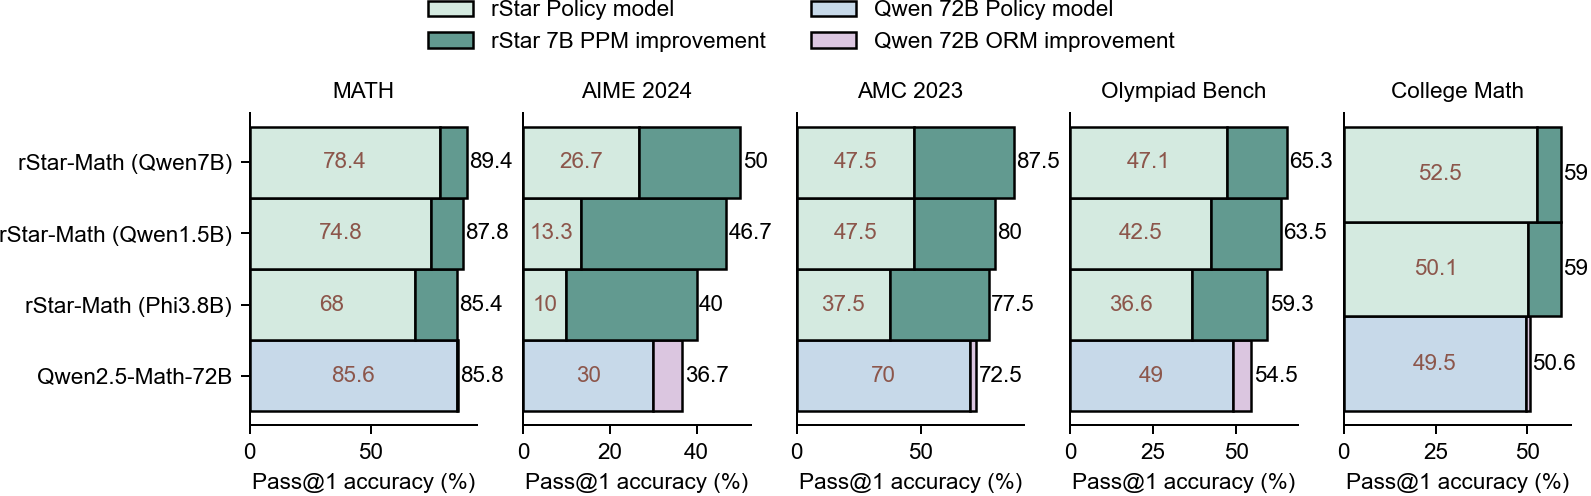
\includegraphics[width=1\textwidth]{ppm_study.png}	
	\vspace{-3ex}
	\caption{Pass@1 accuracy of policy models and their accuracy after applying System 2 reasoning with various reward models, shows that reward models primarily determine the final performance.}
	\label{fig:ppmstudy}
\end{figure*}

 
 
 


  \noindent\textbf{PPM shapes the reasoning boundary in System 2 deep thinking}. Both the policy and reward models are crucial for System 2 deep reasoning. Our experiments show that once the policy model attains a reasonably strong capability level, 
 (see Appendix~\ref{sec:appendexp} ), the PPM becomes the key determinant of the upper performance limit.
   Fig.~\ref{fig:ppmstudy} summarizes the  accuracy of policy models of different sizes, as well as the improvements achieved with reward models. Despite variations in Pass@1 accuracy due to differences in training strategies, datasets, and model scales, the reward model proves to be the dominant factor in System 2 reasoning. For instance, although the SFT accuracy of {\sysname}-7B is lower than Qwen2.5-Math-72B-Instruct, pairing it with our 7B PPM allows {\sysname} to outperform the 72B policy model with Qwen 72B ORM. Moreover, despite varying Pass@1 accuracy across our three policy SLM sizes, the final reasoning accuracy converges after applying the PPM. 
   
   
  

 \noindent\textbf{PPM spots theorem-application steps}. When solving challenging math problems, identifying and applying relevant theorems or key conclusions often form the cornerstone of successful problem-solving~\citep{xin2024deepseek}. In our experiments, we  find that during {\sysname} problem-solving, our PPM effectively identifies critical theorem-application intermediate steps within policy model's deep thinking process. These steps are predicted with high reward scores, guiding the policy model to generate the correct solution. Appendix~\ref{sec:trajectoryexample} provides examples where the PPM successfully identifies key theorems such as Fermat's little theorem~\citep{fermattheorem}, Vieta's formulas~\citep{vietaformula}, the AM-GM inequality~\citep{amgm}, the Pythagorean theorem~\citep{pythagorean-theorem}, and the Shoelace Theorem~\citep{shoelace-theorem}, etc. 
 

  
  
  
  
\noindent\textbf{Generalization discussions}. 
{\sysname} offers a general methodology for improving LLM reasoning applicable to various domains. First, 
 {\sysname} can generalize to more challenging math tasks, such as theorem proving, though its current focus is on word problems due to dataset limitations. Nonetheless, {\sysname} demonstrates the potential to prove  mathematical statements. As shown in Appendix~\ref{sec:trajectoryexample}, it successfully proves an Olympiad-level problem involving Fermat's Little Theorem, providing a step-by-step correct proof through its deep reasoning process. Second, \sysname can generalize to other domains, such as code and commonsense reasoning. Notably, synthesizing step-by-step verified training trajectories for general reasoning requires a mechanism to provide feedback on whether a given trajectory reaches the desired output at the end of MCTS rollout.  For instance, in code reasoning, this could involve designing extensive test cases; in general reasoning, feedback could be obtained through human labeling or mutual verification with another LLM~\citep{rstar}.

 
